\documentclass[11pt,a4paper]{report}
\usepackage[top=1in, bottom=1.5in, left=1in, right=1in]{geometry}
\usepackage[utf8]{inputenc}
\usepackage{amsmath}
\usepackage{amsfonts}
\usepackage{amssymb}
\usepackage[spanish,activeacute]{babel}
\usepackage{multirow}
\usepackage{graphicx}
\usepackage{setspace}
\usepackage{color}
\definecolor{red}{rgb}{1,0,0}
\newcommand\red[1]{\textcolor{red}{#1}}
\newcommand{\dsum}{\displaystyle\sum}

\begin{document}

\setlength{\unitlength}{1 cm} %Especificar unidad de trabajo
\thispagestyle{empty}
\begin{picture}(18,4)
\put(0,0){
\includegraphics[width=2.3cm,height=3cm]{LOGO.jpg}}
%\put(11.5,0){\includegraphics[width=4cm,height=4cm]{eupinf.jpg}}
\end{picture}
\begin{center}
\textbf{{\LARGE Universidad de Concepci\'on}}\\[0.5cm]
{\Large Facultad de Ciencias F\'isicas y Matem\'aticas}\\[0.5cm]
{\Large Departamento de Estad\'istica}\\[3.5cm]
{\LARGE \textbf{LABORATORIO III}}\\[1cm]
{\LARGE \textbf{DATA MINING}}\\ [4cm]
{\large Nombres: Katerin De la hoz Luna}\\
\hspace{2.2cm}{\large Fernando Pe\~na Villalobos}\\
\hspace{1.7cm}{\large Ariel P\'erez Almonacid}\\[2cm]

{\large Concepci\'on \\
\today}
\end{center}

\newpage



\hfill \newline
\begin{itemize}
\item[ Ejercicio 1.]
\item[1.1)] Se procede utilizando el comando rattle(), importando la tabla señalada en la pestaña datos, especificando los separadores, los decimales, cuánto porcentaje ocuparemos para el aprendizaje, cuánto para probar, cuál es nuestra variable a predecir (en este caso chd, es decir, si el paciente sufre o no una enfermedad coronaria) y apretando Ejecutar; resultando lo siguiente:
\begin{center}
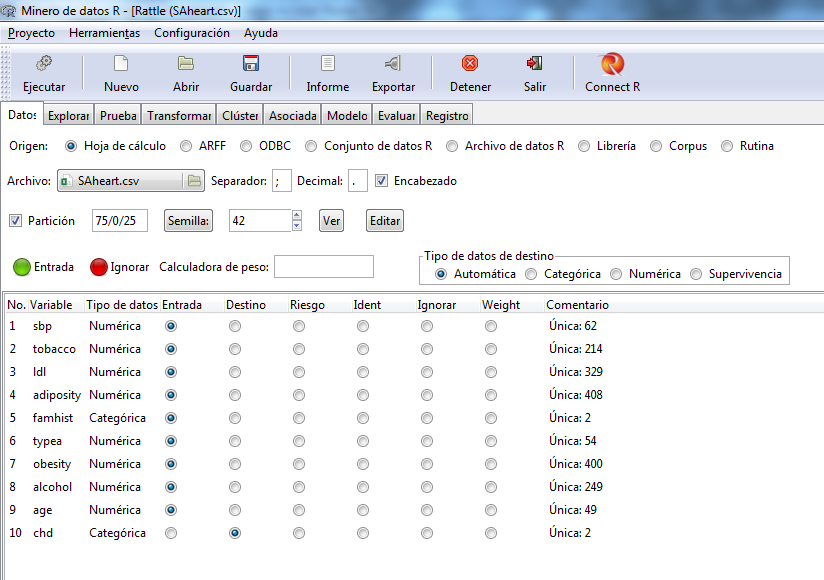
\includegraphics[scale=0.6]{3-1.png}
\end{center}
Cambiando a la pestaña Modelo, seleccionando Árbol y nuevamente presionando en Ejecutar, lo que se entrega es: 
\begin{verbatim}
Resumen del modelo Árbol de decisión de Clasificación (construido con 'rpart'):

n= 346 

node), split, n, loss, yval, (yprob)
      * denotes terminal node

  1) root 346 120 No (0.65317919 0.34682081)  
    2) age< 30.5 86   6 No (0.93023256 0.06976744) *
    3) age>=30.5 260 114 No (0.56153846 0.43846154)  
      6) famhist=Absent 140  41 No (0.70714286 0.29285714)  
       12) tobacco< 7.97 114  26 No (0.77192982 0.22807018)  
         24) sbp< 135 55   6 No (0.89090909 0.10909091) *
         25) sbp>=135 59  20 No (0.66101695 0.33898305)  
           50) alcohol>=26.63 12   0 No (1.00000000 0.00000000) *
           51) alcohol< 26.63 47  20 No (0.57446809 0.42553191)  
            102) typea< 52.5 21   4 No (0.80952381 0.19047619) *
            103) typea>=52.5 26  10 Si (0.38461538 0.61538462) *
       13) tobacco>=7.97 26  11 Si (0.42307692 0.57692308)  
         26) adiposity>=28.87 16   7 No (0.56250000 0.43750000) *
         27) adiposity< 28.87 10   2 Si (0.20000000 0.80000000) *
      7) famhist=Present 120  47 Si (0.39166667 0.60833333)  
       14) ldl< 7.985 110  47 Si (0.42727273 0.57272727)  
         28) tobacco< 12.24 102  47 Si (0.46078431 0.53921569)  
           56) ldl< 5.1 56  24 No (0.57142857 0.42857143)  
            112) adiposity>=23.955 35   8 No (0.77142857 0.22857143) *
            113) adiposity< 23.955 21   5 Si (0.23809524 0.76190476) *
           57) ldl>=5.1 46  15 Si (0.32608696 0.67391304)  
            114) obesity< 24.87 9   2 No (0.77777778 0.22222222) *
            115) obesity>=24.87 37   8 Si (0.21621622 0.78378378)  
              230) tobacco< 6.5 27   8 Si (0.29629630 0.70370370)  
                460) alcohol>=13.5 7   2 No (0.71428571 0.28571429) *
                461) alcohol< 13.5 20   3 Si (0.15000000 0.85000000) *
              231) tobacco>=6.5 10   0 Si (0.00000000 1.00000000) *
         29) tobacco>=12.24 8   0 Si (0.00000000 1.00000000) *
       15) ldl>=7.985 10   0 Si (0.00000000 1.00000000) *

Classification tree:
rpart(formula = chd ~ ., data = crs$dataset[crs$train, c(crs$input, 
    crs$target)], method = "class", parms = list(split = "information"), 
    control = rpart.control(usesurrogate = 0, maxsurrogate = 0))

Variables actually used in tree construction:
[1] adiposity age    alcohol   famhist   ldl   obesity   sbp   tobacco   typea    

Root node error: 120/346 = 0.34682

n= 346 

        CP nsplit rel error  xerror     xstd
1 0.108333      0   1.00000 1.00000 0.073778
2 0.039583      2   0.78333 0.85000 0.070677
3 0.033333      7   0.58333 0.87500 0.071266
4 0.016667      8   0.55000 0.87500 0.071266
5 0.012500     12   0.48333 0.86667 0.071073
6 0.010000     14   0.45833 0.85000 0.070677

Tiempo transcurrido: 0.06 segs

\end{verbatim}
\item[1.2)] Para calcular la matriz de confusión, se cambia a la pestaña Evaluar, marcando en Matriz de Error y en Árbol, el cual es el modelo con el que se está trabajando, y nuevamente se ejecuta, dando como resultado la siguiente matriz de confusión:

$$\begin{tabular}{| c |  r l  r |}
\hline
  & & Predicho&  \\
   \hline
     &  & No& Si \\
 Real& No   &55 &21 \\
     & Si   &24 & 16\\
   \hline
 \end{tabular} $$

De donde se puede extraer la siguiente información:\\
Precisión Global = $61\%$\\
Precisión Positiva = $40\%$\\
Precisión Negativa = $72\%$\\
Falsos Positivos = $28\%$\\
Falsos Negativos = $60\%$\\

\item[1.3)] Volviendo a la pestaña Modelo se aprieta el botón Dibujar para ver el árbol de decisión generado y Reglas para ver las reglas de decisión.
\begin{center}
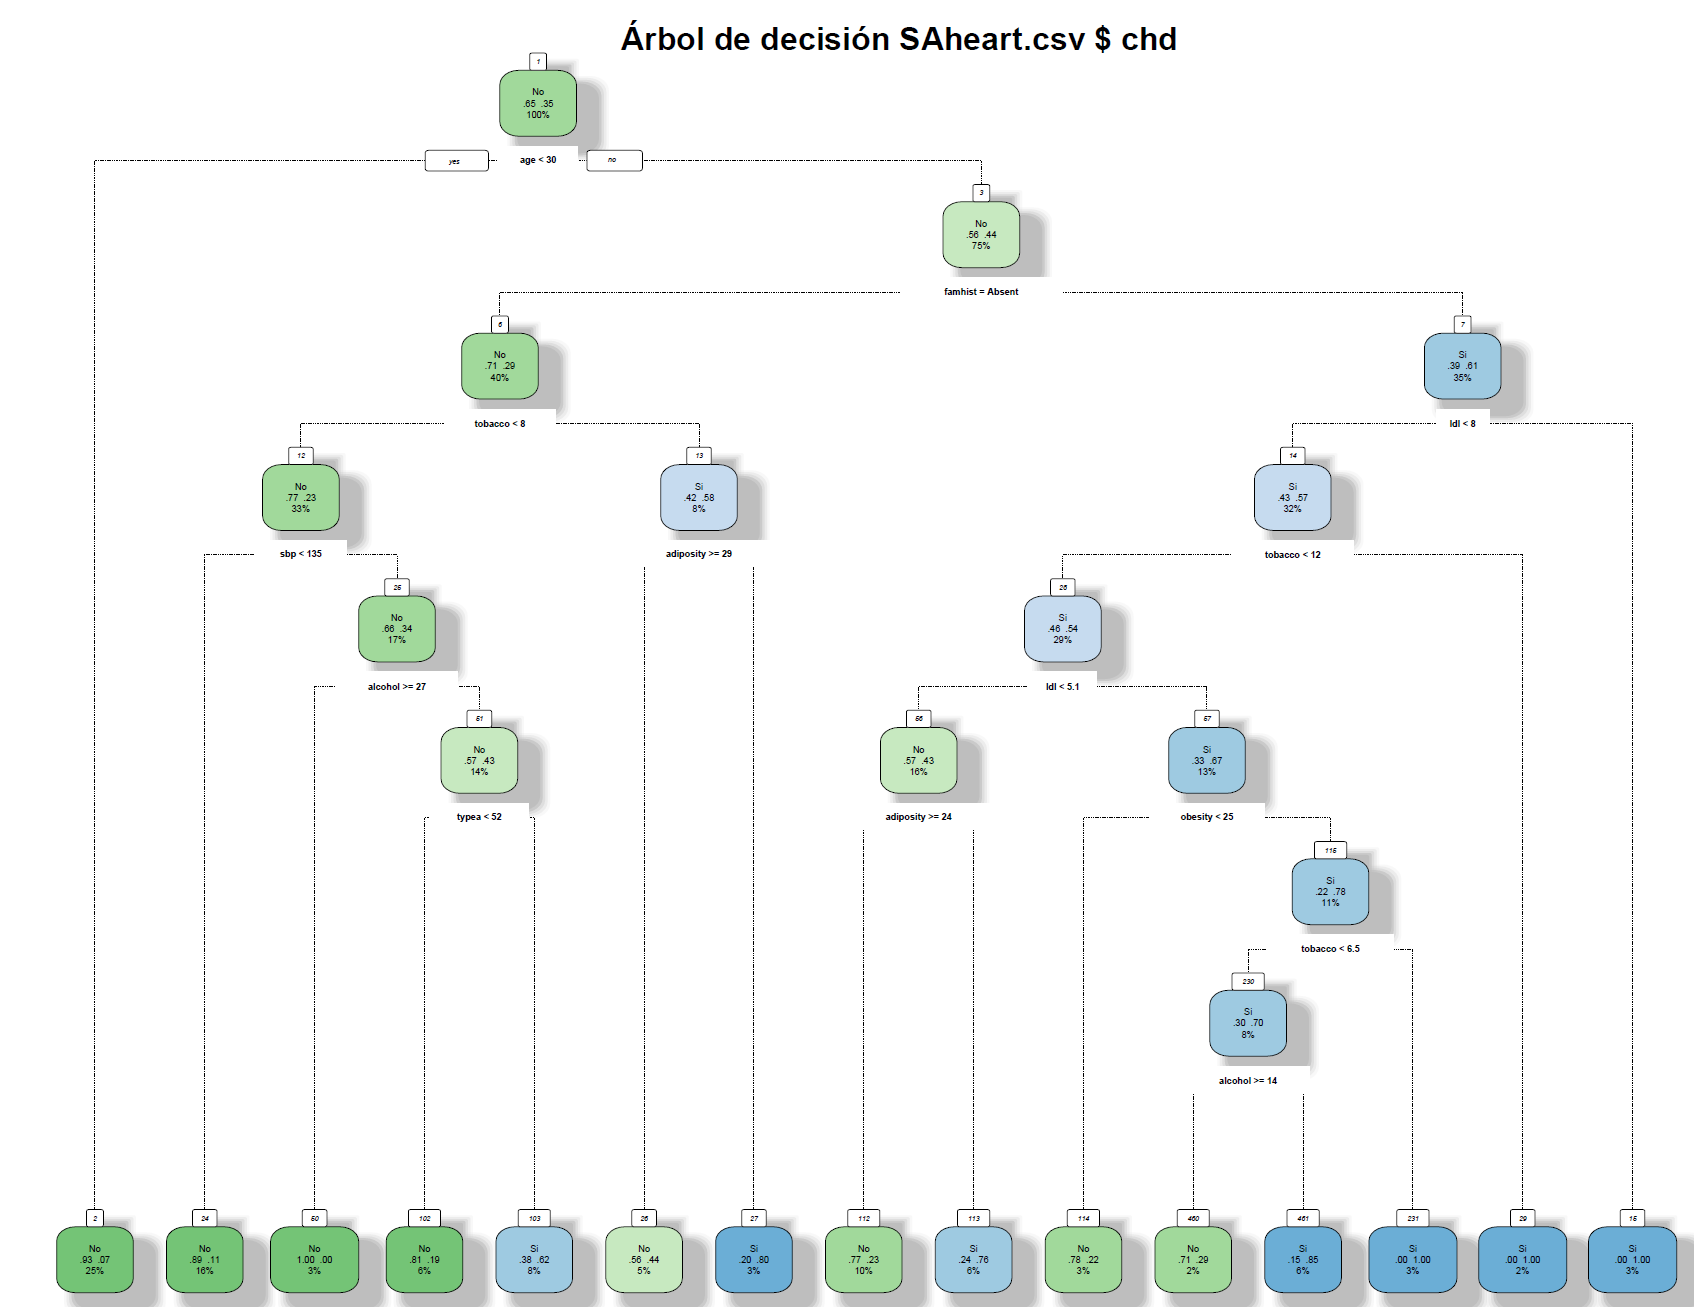
\includegraphics[scale=0.35]{arbol.png}
\end{center}

\begin{verbatim}
 Rule number: 15 [chd=Si cover=10 (3%) prob=1.00]
   age>=30.5
   famhist=Present
   ldl>=7.985

 Rule number: 29 [chd=Si cover=8 (2%) prob=1.00]
   age>=30.5
   famhist=Present
   ldl< 7.985
   tobacco>=12.24

 Rule number: 231 [chd=Si cover=10 (3%) prob=1.00]
   age>=30.5
   famhist=Present
   ldl< 7.985
   tobacco< 12.24
   ldl>=5.1
   obesity>=24.87
   tobacco>=6.5

 Rule number: 461 [chd=Si cover=20 (6%) prob=0.85]
   age>=30.5
   famhist=Present
   ldl< 7.985
   tobacco< 12.24
   ldl>=5.1
   obesity>=24.87
   tobacco< 6.5
   alcohol< 13.5

 Rule number: 27 [chd=Si cover=10 (3%) prob=0.80]
   age>=30.5
   famhist=Absent
   tobacco>=7.97
   adiposity< 28.87

 Rule number: 113 [chd=Si cover=21 (6%) prob=0.76]
   age>=30.5
   famhist=Present
   ldl< 7.985
   tobacco< 12.24
   ldl< 5.1
   adiposity< 23.95

 Rule number: 103 [chd=Si cover=26 (8%) prob=0.62]
   age>=30.5
   famhist=Absent
   tobacco< 7.97
   sbp>=135
   alcohol< 26.63
   typea>=52.5

 Rule number: 26 [chd=No cover=16 (5%) prob=0.44]
   age>=30.5
   famhist=Absent
   tobacco>=7.97
   adiposity>=28.87

 Rule number: 460 [chd=No cover=7 (2%) prob=0.29]
   age>=30.5
   famhist=Present
   ldl< 7.985
   tobacco< 12.24
   ldl>=5.1
   obesity>=24.87
   tobacco< 6.5
   alcohol>=13.5

 Rule number: 112 [chd=No cover=35 (10%) prob=0.23]
   age>=30.5
   famhist=Present
   ldl< 7.985
   tobacco< 12.24
   ldl< 5.1
   adiposity>=23.95

 Rule number: 114 [chd=No cover=9 (3%) prob=0.22]
   age>=30.5
   famhist=Present
   ldl< 7.985
   tobacco< 12.24
   ldl>=5.1
   obesity< 24.87

 Rule number: 102 [chd=No cover=21 (6%) prob=0.19]
   age>=30.5
   famhist=Absent
   tobacco< 7.97
   sbp>=135
   alcohol< 26.63
   typea< 52.5

 Rule number: 24 [chd=No cover=55 (16%) prob=0.11]
   age>=30.5
   famhist=Absent
   tobacco< 7.97
   sbp< 135

 Rule number: 2 [chd=No cover=86 (25%) prob=0.07]
   age< 30.5

 Rule number: 50 [chd=No cover=12 (3%) prob=0.00]
   age>=30.5
   famhist=Absent
   tobacco< 7.97
   sbp>=135
   alcohol>=26.63
\end{verbatim}
\end{itemize}

\begin{itemize}
\item[Ejercicio 2.] 
\item[2.1)] Se usa la interfaz rattle() con la tabla de datos dada de forma análoga a cómo se describió en el Ejercicio 1, usando 70\% de los datos de los datos para la tabla de aprendizaje y 30\% para la tabla de prueba.
\item[2.2)]Usando Árboles de decisión, se obtiene la siguiente matriz de confusión, para la variable PurchasedBike
$$\begin{tabular}{| c |  r l  r |}
\hline
  & & Predicho&  \\
   \hline
     &  & No& Si \\
 Real& No   &352 &167 \\
     & Si   & 144& 337\\
   \hline
 \end{tabular} $$
Y la matriz de error :
$$\begin{tabular}{| c |  r l  r |}
\hline
  & & Predicho&  \\
   \hline
     &  & No& Si \\
 Real& No   &0.35 &0.17 \\
     & Si   & 0.14& 0.34\\
   \hline
 \end{tabular} $$
De donde se puede extraer la siguiente información:\\
Precisión Global: $69\%$\\
Precisión Positiva: $70\%$\\
Precisión Negativa: $67\%$\\
Falsos Positivos: $33\%$ \\
Falsos Negativos: $30\%$\\
Se aprecia que la precisión positiva y la precisión negativa es alta, con lo cual el método es aceptable para identificar a quienes van a comprar y a quienes no van a comprar bicicletas. Ya que los árboles de decisión permiten identificar las características que determinaron la clasificación de un cliente, este método podría ser útil para una empresa, ya sea para crear estrategias que permitan captar clientes nuevos, o para introducir nuevos productos para clientes existentes.

\item[2.3)] Se tiene el siguiente árbol de decisión:
\begin{center}
\includegraphics[scale=0.5]{Rplot01.png}
\end{center}

Y la lista de las reglas de decisión
\begin{verbatim}
Rule number: 29 [PurchasedBike=Yes cover=17 (2%) prob=0.82]
   Cars< 1.5
   Age< 54.5
   Age< 32.5
   CommuteDistance=0-1Miles

 Rule number: 95 [PurchasedBike=Yes cover=68 (10%) prob=0.71]
   Cars>=1.5
   Income>=3.5e+04
   Children< 4.5
   CommuteDistance=0-1Miles,2-5Miles,5-10Miles
   Education=Bachelors,PartialCollege
   Age>=32.5

 Rule number: 15 [PurchasedBike=Yes cover=268 (38%) prob=0.68]
   Cars< 1.5
   Age< 54.5
   Age>=32.5

 Rule number: 46 [PurchasedBike=No cover=59 (8%) prob=0.42]
   Cars>=1.5
   Income>=3.5e+04
   Children< 4.5
   CommuteDistance=0-1Miles,2-5Miles,5-10Miles
   Education=GraduateDegree,HighSchool,PartialHighSchool

 Rule number: 22 [PurchasedBike=No cover=85 (12%) prob=0.34]
   Cars>=1.5
   Income>=3.5e+04
   Children< 4.5
   CommuteDistance=1-2Miles,10+Miles

 Rule number: 28 [PurchasedBike=No cover=40 (6%) prob=0.28]
   Cars< 1.5
   Age< 54.5
   Age< 32.5
   CommuteDistance=1-2Miles,2-5Miles,5-10Miles

 Rule number: 6 [PurchasedBike=No cover=37 (5%) prob=0.27]
   Cars< 1.5
   Age>=54.5

 Rule number: 4 [PurchasedBike=No cover=72 (10%) prob=0.21]
   Cars>=1.5
   Income< 3.5e+04

 Rule number: 10 [PurchasedBike=No cover=47 (7%) prob=0.19]
   Cars>=1.5
   Income>=3.5e+04
   Children>=4.5

 Rule number: 94 [PurchasedBike=No cover=7 (1%) prob=0.14]
   Cars>=1.5
   Income>=3.5e+04
   Children< 4.5
   CommuteDistance=0-1Miles,2-5Miles,5-10Miles
   Education=Bachelors,PartialCollege
   Age< 32.5

\end{verbatim}

\end{itemize}	

\begin{itemize}
\item[Ejercicio 3.] 
\item[3.1)] El tiempo de ejecución del algoritmo es $17.9$ seg. Este tiempo es razonable si se piensa en implementar el algoritmo en una oficina de correos.
\item[3.2)] A continuación se tiene la matriz de confusión: 
$$\begin{tabular}{|l| c c c c c c c c c c c|} 
\hline 
& & & & &\multicolumn{7}{l|}{Predicho}\\
\hline 
 & & cero & cinco & cuatro & dos & nueve & ocho & seis & siete & tres & uno \\
 & cero & 297 & 1 & 1 & 33 & 2 & 13 & 2 & 0 & 9 & 1 \\
 & cinco & 18 & 87 & 2 & 7 & 9 & 6 & 11 & 2 & 15 & 3 \\
 & cuatro & 1 & 1 & 138 & 13 & 23 & 3 & 0 & 5 & 0 & 16\\
 & dos & 9 & 2 & 12 & 108 & 12 & 25 & 13 & 5 & 10 & 2\\
Real & nueve & 0 & 0 & 0 & 4 & 149 & 5 & 0 & 8 & 5 & 6\\  
 & ocho & 2 & 3 & 2 & 14 & 13 & 115 & 3 & 2 & 11 & 1\\
 & seis & 11 & 9 & 2 & 5 & 1 & 24 & 107 & 3 & 1 & 7\\
 & siete & 1 & 0 & 10 & 5 & 13 & 4 & 0 & 113 & 1 & 0\\
 & tres & 12 & 22 & 2 & 4 & 3 & 15 & 0 & 3 & 102 & 3\\
 & uno  & 1 & 1 & 3 & 1 & 8 & 6 & 0 & 1 & 0 & 243 \\
\hline
\end{tabular} $$
Se recuerda que la precisión global es la proporción de casos que fueron identificados correctamente y la precisión positiva es la proporción de casos positivos que fueron identificados correctamente. En nuestro caso, la precisión global es 73\%, y las precisiones positivas para cada número son las siguientes:
$$\begin{tabular}{|l c |l c|}
\hline
cero & 0.827 & ocho & 0.693 \\
cinco & 0.544 & seis & 0.629 \\
cuatro & 0.690 & siete & 0.769 \\
dos & 0.545 & tres & 0.614\\
nueve & 0.842 & uno & 0.920 \\
\hline
\end{tabular}$$
Si bien, la precisión es alta, lo ideal sería que bordeara el 90\% para pensar en implementar el método en una oficina de correos, pues no sería eficiente ni conveniente para la oficina que de 100 cartas, 27 fueran enviadas erronemente. \\ Como lo que importa es saber que tan bien se detectan los números, se analiza la precisión positiva. Ésta fue baja para el cinco, el dos, el tres y el seis, lo cual se debe al parecido que tienen ciertos números. El cinco se confunde con el cero, el tres y el seis; el dos con ocho, el seis, el cuatro y el nueve; el tres con el cinco, el cero y el ocho; y finalmente, el seis con el ocho, el cero y el cinco. 
\item[3.3)] El gráfico del árbol de decisión generado es:
\begin{center}
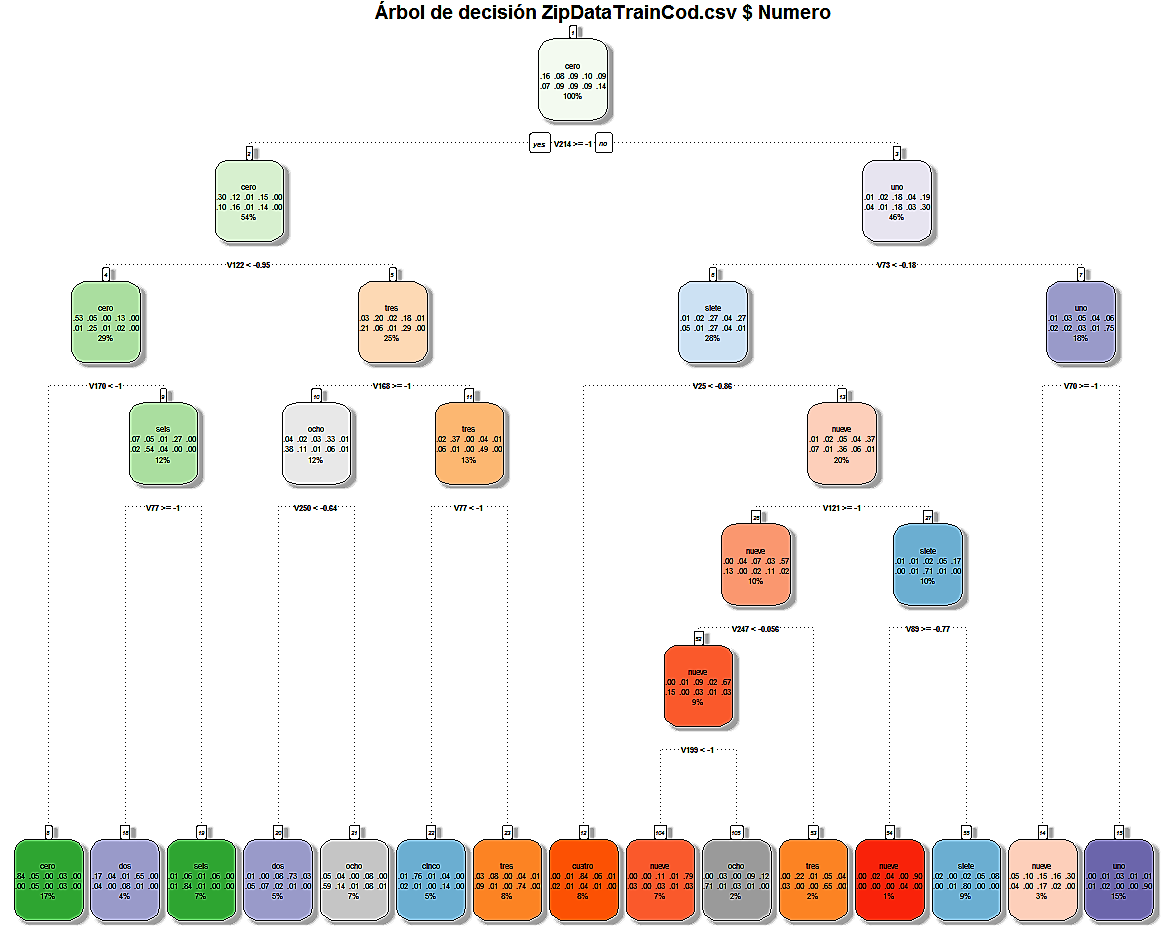
\includegraphics[scale=0.5]{arbol3.png}
\end{center}
Y la lista de reglas de cuadratura es:
\begin{verbatim}
 Rule number: 20 [Numero=dos cover=332 (5%) prob=242.00]
   V214>=-0.9995
   V122>=-0.9535
   V168>=-0.9995
   V250< -0.6425

 Rule number: 18 [Numero=dos cover=311 (4%) prob=202.00]
   V214>=-0.9995
   V122< -0.9535
   V170>=-0.9995
   V77>=-0.9995

 Rule number: 21 [Numero=ocho cover=538 (7%) prob=45.00]
   V214>=-0.9995
   V122>=-0.9535
   V168>=-0.9995
   V250>=-0.6425

 Rule number: 14 [Numero=nueve cover=221 (3%) prob=36.00]
   V214< -0.9995
   V73>=-0.1815
   V70>=-0.9965

 Rule number: 55 [Numero=siete cover=653 (9%) prob=35.00]
   V214< -0.9995
   V73< -0.1815
   V25>=-0.862
   V121< -0.9995
   V89< -0.775

 Rule number: 12 [Numero=cuatro cover=563 (8%) prob=35.00]
   V214< -0.9995
   V73< -0.1815
   V25< -0.862

 Rule number: 8 [Numero=cero cover=1255 (17%) prob=35.00]
   V214>=-0.9995
   V122< -0.9535
   V170< -0.9995

 Rule number: 19 [Numero=seis cover=545 (7%) prob=32.00]
   V214>=-0.9995
   V122< -0.9535
   V170>=-0.9995
   V77< -0.9995

 Rule number: 23 [Numero=tres cover=558 (8%) prob=20.00]
   V214>=-0.9995
   V122>=-0.9535
   V168< -0.9995
   V77>=-0.9975

 Rule number: 22 [Numero=cinco cover=400 (5%) prob=15.00]
   V214>=-0.9995
   V122>=-0.9535
   V168< -0.9995
   V77< -0.9975

 Rule number: 15 [Numero=uno cover=1086 (15%) prob=13.00]
   V214< -0.9995
   V73>=-0.1815
   V70< -0.9965

 Rule number: 105 [Numero=ocho cover=117 (2%) prob=11.00]
   V214< -0.9995
   V73< -0.1815
   V25>=-0.862
   V121>=-0.9995
   V247< -0.0555
   V199>=-0.9975

 Rule number: 53 [Numero=tres cover=112 (2%) prob=6.00]
   V214< -0.9995
   V73< -0.1815
   V25>=-0.862
   V121>=-0.9995
   V247>=-0.0555

 Rule number: 104 [Numero=nueve cover=518 (7%) prob=4.00]
   V214< -0.9995
   V73< -0.1815
   V25>=-0.862
   V121>=-0.9995
   V247< -0.0555
   V199< -0.9975

 Rule number: 54 [Numero=nueve cover=82 (1%) prob=0.00]
   V214< -0.9995
   V73< -0.1815
   V25>=-0.862
   V121< -0.9995
   V89>=-0.775
\end{verbatim}
\end{itemize}
\begin{itemize}
\item[Ejercicio 4.] 
\item[4.1)] Información ganada usando el Índice de Gini.\\

\underline{Primera división}: Primero, se calcula P(i), para cada nodo, que es la probabilidad de estar en la clase i.\\

Nodo 1: P(A) = $\frac{62}{70}$, P(B) = $\frac{8}{70}$, P(C) = $0$ \\

Gini(1) = $1-(\frac{62}{70})^2-(\frac{8}{70})^2 = 0.2$  \\

Nodo 2: P(A) = $\frac{38}{140}$, P(B) = $\frac{42}{140}$, P(C) = $\frac{60}{140}$ \\

Gini(2) = $1-(\frac{38}{140})^2-(\frac{42}{140})^2 - (\frac{60}{140})^2 =0.65$ \\

Se calcula Gini$_{split}=(\frac{70}{210})*0.20 + (\frac{140}{210})*0.65 = 0.5$\\

\underline{Segunda división}: \\

Nodo 1: P(A) = $\frac{65}{85}$, P(B) = $\frac{20}{85}$, P(C) = $0$ \\

Gini(1) = $1-(\frac{65}{85})^2-(\frac{20}{85})^2 = 0.36$ \\

Nodo 2: P(A) = $\frac{21}{60}$, P(B) = $\frac{19}{60}$, P(C) = $\frac{20}{60}$ \\

Gini(2) = $1-(\frac{21}{60})^2-(\frac{19}{60})^2 - (\frac{20}{60})^2 =0.67$ \\

Nodo 3: P(A) = $\frac{14}{65}$, P(B) = $\frac{11}{65}$, P(C) = $\frac{40}{65}$ \\

Gini(3) = $1-(\frac{14}{65})^2-(\frac{11}{65})^2 - (\frac{40}{65})^2 =0.55$ \\

Se calcula Gini$_{split}=(\frac{85}{210})*0.36 + (\frac{60}{210})*0.67 + (\frac{65}{210})*0.55 = 0.51$\\

A partir de lo anterior, se debe escoger la primera división, pues tiene menor Gini$_{split}$, lo que maximiza la información ganada.

\item[4.2)] Información ganada usando Entropía. \\

\underline{Primera división}: Se calcula la entropía para cada nodo. \\

Entropía(1)= $-(\frac{62}{70})\log_2(\frac{62}{70})-(\frac{8}{70})\log_2(\frac{8}{70}) = 0.51$\\

Entropía(2)= $-(\frac{38}{140})\log_2(\frac{38}{140})-(\frac{42}{140})\log_2(\frac{42}{140}) - (\frac{60}{140})\log_2(\frac{60}{140}) =1.56$\\

Se calcula Entropía$_{split}=(\frac{70}{210})*0.51 + (\frac{140}{210})*1.56 = 1.21$\\ 

\underline{Segunda división}: \\

Entropía(1) = $-(\frac{65}{85})\log_2(\frac{65}{85})-(\frac{20}{85})\log_2(\frac{20}{85}) = 0.79$ \\

Entropía(2)=$-(\frac{21}{60})\log_2(\frac{21}{60})-(\frac{19}{60})\log_2(\frac{19}{60}) - (\frac{20}{60})\log_2(\frac{20}{60})=1.58$\\

Entropía(3) = $-(\frac{14}{65})\log_2(\frac{14}{65})-(\frac{11}{65})\log(\frac{11}{65}) - (\frac{40}{65})\log_2(\frac{40}{65}) =1.34$ \\

Se calcula Entropía$_{split}=(\frac{85}{210})*0.79 + (\frac{60}{210})*1.58 + (\frac{65}{210})*1.34 = 1.19$\\  

Entonces, se escoge la segunda división, pues minimiza la Entropía$_{split}$, lo cual maximiza la información ganada.

\item[4.3)] Información ganada usando Error de Clasificación.\\

\underline{Primera división}:\\

EC(1)$=1-\frac{62}{70}=0.11$ \\

EC(2)$=1-\frac{60}{140}=0.57$\\

Se calcula EC$_{split}=(\frac{70}{210})*0.11 + (\frac{140}{210})*0.57 = 0.42$\\

\underline{Segunda división}:\\

EC(1)$=1-\frac{65}{85}=0.24$\\

EC(2)$=1-\frac{21}{60}=0.65$\\

EC(3)$=1-\frac{40}{65}=0.39$\\

Se calcula EC$_{split}=(\frac{85}{210})*0.24 + (\frac{60}{210})*0.65 + (\frac{65}{210})*0.39 = 0.40$\\

La mejor división es la segunda, pues minimiza EC$_{split}$ con lo cual, se maximiza la información ganada.

\end{itemize}


\end{document}
